\chapter{Introduction}\label{ch:intro}

\begin{draftnote}
Drafted 2026-08-02, expanded 2026-08-03, revised twice more on 2026-08-03. Citations follow the
Chapter 1 rows of the claim map in \texttt{logbook/10\_references.md}.

\textbf{Third pass (audit fixes).} The chapter previously described the experiment two
incompatible ways: \S1.2 named the three arms as baseline / control / constrained, while \S1.4
named them as baseline plus two constrained variants at different budgets. \S1.4 matched the
locked scope in \texttt{CLAUDE.md} and \S1.2 did not. \S1.2 is now rewritten to explain why the
control arm exists without committing to a count, to record that the control arm reproduced the
baseline exactly (so the two collapse into one reported arm), and to name both cost budgets, 25
and 15. Objectives gained the second budget, now say five seeds instead of "multiple", and end on
an outcome-framed objective rather than four activity-framed ones. Also fixed: \(\pi\) now set as
maths, a clause added explaining why the book's title is narrower than the registered title, and
four low-value "not X" constructions rewritten positively.

\textbf{Second pass.} Dropped the "1.1" heading from the platform material so it reads as unheaded
opening paragraphs (sections renumber automatically, Background is now 1.1); added a paragraph on
where UR5e-class arms are actually used; converted the two Problem Description issues into a
labelled list; and widened Scope (full registered title, what Layers 2/3 would technically have
covered, and a positioning sentence on constrained RL as existing robotics practice), using only
citations already in \texttt{references.bib}, no new sources, per Touhid's choice.

\cite{shen2022reactive} and \cite{altman1999cmdp} are licensed for this chapter too (the
reward-vs-constraint framing and the CMDP tuple respectively) but are deliberately left to
Chapter~\ref{ch:litreview}, which already carries both in full, \cite{shen2022reactive} at \S2.6
and \cite{altman1999cmdp} at \S2.3. Flag to Touhid if he wants either pulled forward.

\textbf{Open item, not fixed here:} Chapter~\ref{ch:litreview} \S2.1 is close to word-for-word the
reserved prose this chapter was originally drafted from, not a forward-pointer to it. The two
chapters still overlap in their framing paragraphs. Worth a trim pass on \S2.1 once Chapter 1 is
settled, but that is Touhid's call.

\textbf{Photo status:} \texttt{figures/ur5e\_platform\_interim.png} is a placeholder, an extracted
photograph from \cite{xia2024proactive}, credited in the caption below, not an original
photograph of this project. Swap it for Touhid's own UR5e photograph when supplied; instructions
for the swap are in \texttt{Thesis\_LaTeX/figures/README.md}.
\end{draftnote}

A manipulator is, in its simplest description, a chain of rigid links connected by powered
joints, ending in a tool that does the actual work of picking something up, placing it, or
holding it against a process. For most of industrial robotics' history this chain worked alone,
fenced off from people, repeating a single memorised path thousands of times a shift. The
collaborative arm changes that arrangement: it is built to share a workspace with a person, which
means every motion it makes must be treated as something that could come near a hand, not just
near a workpiece. This thesis is built around one specific arm of that kind, and the platform is
not incidental to the argument. Everything the simulation trains against, from the joint speeds
it is allowed to command to the distances it is allowed to close, is set to match what this
particular machine can actually do.

\begin{kuetfigure}[H]{A UR5e collaborative arm sharing a workspace with a person. Photograph
reproduced from Xia et al. \cite{xia2024proactive}, Fig.~1, under that paper's CC BY-NC-ND 4.0
licence. Placeholder pending an original photograph of the platform used in this project.}{fig:i-ur5e-photo}
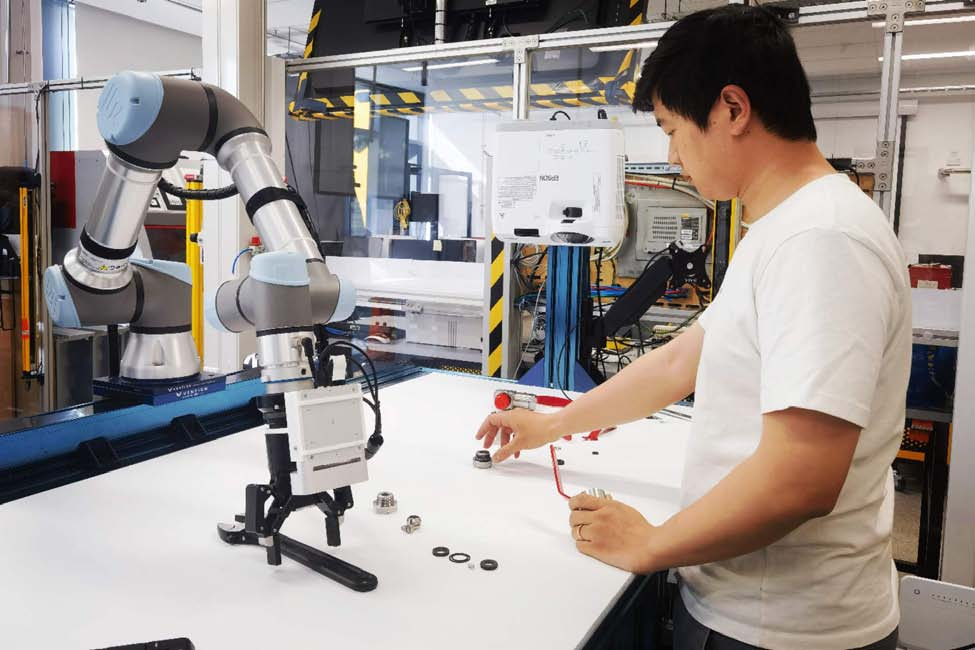
\includegraphics[width=0.72\textwidth]{figures/ur5e_platform_interim.png}
\end{kuetfigure}

The platform is a Universal Robots UR5e, a six-joint (6-DOF) collaborative arm
\cite{universalrobots2023ur5e}. It carries a payload of 5 kg to a reach of 850 mm, repeats a
taught position to within 0.03 mm, and weighs 20.6 kg unmounted. Every one of its six joints is
rated to the same maximum speed, 180 deg/s, which is exactly \(\pi\) rad/s. The simulated
arm in this thesis is capped at 3.14 rad/s for the same reason a real one is: past that speed the
motion stops being something a person nearby could react to in time. The provenance of that figure
matters: 3.14 rad/s is the datasheet limit itself, carried into the simulator so that a policy
trained there is never asked to move faster than the physical machine could follow it. The UR5e also ships with seventeen configurable safety
functions and is certified to the relevant collaborative-robot safety standards, ISO 13849-1
(Category 3, Performance Level d) and ISO 10218-1 \cite{universalrobots2023ur5e}. None of those
seventeen functions is exercised by the simulation. What this thesis borrows from the platform is
its physical envelope, its speed and reach limits, not its built-in safety controller, and
Chapter~\ref{ch:methods} is explicit about which of the two is under test.

Machines with this specification already do real work outside the laboratory. UR-class arms in
the UR5e's size class are common on production floors for exactly the tasks a 5 kg payload and an
850 mm reach suit: pick-and-place, machine tending, small-parts assembly and packaging, and
inspection stations where a part has to be picked up and held in front of a camera. The same
collaborative certification that lets one work next to a person on a line is also why it turns up
so often in research: it is affordable enough for a university laboratory, safety-rated enough to
run near people without a fenced cell, and common enough on real production floors that a result
obtained on one arm should say something useful about the rest of that population. Two of the
papers already cited in this chapter used a UR5-class arm for exactly that reason, one for
grasping \cite{ferreira2025grasping} and one for collision avoidance around a moving person
\cite{xia2024proactive}. The platform used here is drawn from that same working population.

Two further reasons fixed the choice. The preceding project in this laboratory used a
different, custom five-degree-of-freedom arm for classical visual servoing
\cite{khan2025csrt_ibvs}; this thesis moves to a UR-class platform because the safety question it
asks, how a learned policy behaves near a joint limit or a kinematic singularity, is best posed on
hardware whose limits and safety record are already public and well documented. Isaac Lab, the
simulation framework used throughout (Chapter~\ref{ch:methods}), also ships the UR5e as one of its
reference manipulators, so building the environment on this arm meant working from a supported
example rather than adapting a custom robot from scratch. The joint limits and speed ceiling used
throughout this thesis therefore belong to a machine that exists, not one assumed for convenience.

\section{Background}\label{sec:i-background}

Industrial manipulators increasingly work in spaces shared with people rather than behind a
fence, and the UR5e described above is a working example of that shift.
A controller that follows a fixed, hand-derived trajectory can be inspected and bounded before it
ever moves: an engineer can trace every configuration it will visit and check each one against a
joint limit or a known obstacle. A policy obtained by training a reinforcement learning agent
cannot be inspected the same way. Its behaviour is known only through the statistics of the
trajectories it produces during and after training, not through a proof that covers every
configuration it might reach. Safe operation of a UR-class collaborative arm around people is
already treated as a live industrial requirement, not a hypothetical one \cite{xia2024proactive}.
Reinforcement learning is attractive for manipulation precisely because it can learn grasping and
placement behaviour directly from experience, without a hand-built controller for every object and
pose the arm might encounter. What that learned behaviour does in the configurations it visits
rarely, however, is not a detail to be checked after the fact. For a policy sharing a workspace
with a person, it is the condition deployment depends on.

The standard formulation of reinforcement learning gives a designer only one channel for stating
what the agent should avoid: the reward function. Take the UR5e's own joint-speed ceiling as a
concrete case. A designer who wants the trained policy to respect it has, in the standard
formulation, exactly one lever: add a penalty term for exceeding it, sized by a weight that trades
a unit of excess speed against a unit of task reward. That weight has to be fixed before training
starts, before the designer has any real sense of how large a violation the untrained policy will
produce or how much task performance the penalty will cost once it starts to bind. Set the weight
too small and the constraint is decorative. Set it too large and the agent may refuse to move at
all. An alternative, pursued in this thesis, is to keep the requirement outside the reward
entirely and state it instead as a constraint with an explicit budget: a quantity that can be set
from a measurement of the system, such as the arm's own rated limits, and checked afterwards
against what the trained policy actually used \cite{achiam2017cpo}. The distinction matters
because of what each side has to answer for. A reward weight is a guess, tuned by trial and error
against whatever the agent happens to do. A constraint budget is a number the designer can defend
before training ever starts, because it comes from a measurement rather than a hunch.
Chapter~\ref{ch:litreview} reviews this distinction, and the literature built on either side of
it, in full.

\section{Problem Description}\label{sec:i-problem}

This thesis puts that alternative to a direct test. It trains a UR5e in simulation to pick up and
lift a cube, comparing a standard proximal policy optimisation (PPO) agent against a constrained
variant of the same algorithm (PPO-Lagrangian) under a shared floor on manipulability, a measure of
how far a configuration sits from a kinematic singularity. Such a comparison, as usually run in the
literature, has two problems.

\begin{itemize}
  \item \textbf{The cost-critic confound.} Adding a constraint to an RL agent does not add only a
  constraint. A Lagrangian method also adds a cost critic, a second value network trained
  alongside the policy to estimate the constraint violation the current policy would incur. That
  network is present whether or not the constraint is actively binding, and its presence can
  influence training through machinery the two agents no longer share. A comparison that trains
  only the unconstrained baseline and the fully constrained agent cannot separate what the
  constraint achieved from what the extra network alone changed.
  \item \textbf{Seed variance.} A single training run under one random seed says little about what
  a method will do on the next run \cite{henderson2018matters}. Published comparisons of
  constrained against unconstrained manipulation policies typically report one run, or a mean over
  few, without a measure of how much the outcome would vary if the same method were retrained.
\end{itemize}

Section~\ref{sec:b-gap} sets out this gap in full against the closest published comparison
\cite{khan2026rl_precision_grasping}. What matters here is the consequence for design.
Chapter~\ref{ch:methods} describes a comparison built to answer both problems at once. Alongside
the unconstrained baseline it places a control arm, identical to the constrained agent in every
respect except that its Lagrange multiplier is pinned to zero, so that whatever the cost critic
does on its own can be measured apart from whatever the constraint does. The constrained agent is
trained at two episodic cost budgets, 25 and 15, because a tighter budget and a looser one make
different demands of the policy. Every arm is trained on five independent random seeds, and every
reported quantity carries its spread across those seeds instead of standing as a single number.

The control arm turned out to reproduce the unconstrained baseline exactly, at the level of the
stored network weights rather than merely to within statistical noise, so the two are reported
jointly as a single arm throughout Chapter~\ref{ch:results}. The isolation this design was built
to provide therefore measures the cost critic's independent effect as exactly zero, and
Section~\ref{sec:r-validity} gives that verification in full. Three arms are reported in the end:
the joint baseline, and the constrained agent at each of its two budgets.

The work also continues a line of manipulator research from the same laboratory. The preceding
study \cite{khan2025csrt_ibvs} addressed the perception and motion side of manipulation, tracking
and following a target with classical image-based visual servoing. This thesis addresses the
control policy instead, with reinforcement learning, and adds a safety constraint that a classical
visual servoing loop does not itself provide.

\section{Objectives}\label{sec:i-objectives}

The general objective of this thesis is to determine whether expressing a manipulability safety
requirement as an explicit constraint, rather than as a term in the reward, changes the safety
behaviour of a learned grasping policy on a UR5e manipulator, and whether it changes how
predictable that behaviour is across independent training runs.

The specific objectives are as follows:

\begin{itemize}
  \item To implement an unconstrained PPO baseline and a constrained PPO-Lagrangian agent for a
  UR5e pick-and-lift grasping task in Isaac Lab, trained under a shared floor on manipulability.
  \item To isolate the effect of the constraint from the effect of the cost critic that implements
  it, by training a control arm that carries the cost critic with its Lagrange multiplier held at
  zero throughout training.
  \item To establish whether the constrained agent's behaviour depends on how tight its budget is,
  by training it at two episodic cost budgets, 25 and 15, instead of one.
  \item To train every arm on five independent random seeds and report task performance and safety
  outcomes as a distribution across those seeds instead of as a single mean.
  \item To evaluate every trained policy on frozen, held-out episodes, so that the reported safety
  and task figures describe the policy that would actually be deployed rather than a
  still-learning one.
  \item To determine, from the resulting distributions, whether the constraint changes the average
  safety outcome of a training run, the spread of that outcome across runs, or both.
\end{itemize}

\section{Scope}\label{sec:i-scope}

This thesis was registered under the title \textit{Safe Adaptive Image-Based Visual Servoing with
Constrained Reinforcement Learning for Precision Grasping on a UR5 Manipulator: From Simulation to
Real Hardware}, and was proposed as a three-layer programme, not as Layer 1 alone. The title on
this book is narrower because the delivered work is narrower, and the paragraphs below say exactly
where the boundary falls.

Layer 1, delivered here, is safe reinforcement learning for grasping in simulation, using
privileged pose information rather than vision. Layer 2 would have closed the loop with vision: an
image-based visual servoing scheme in which the image Jacobian relating pixel motion to joint
motion is tuned by the learned policy rather than fixed in advance, replacing the privileged pose
feedback of Layer 1 with an eye-in-hand RGB-D camera and object detection. It would have been a
direct upgrade of the predecessor project in this laboratory, which used a fixed, hand-derived
image Jacobian for the same visual-servoing task \cite{khan2025csrt_ibvs}. Layer 3 would have
carried the resulting controller onto the physical UR5e over ROS 2, closing the gap between the
Robotiq 2F-85 gripper modelled in simulation and the different gripper fitted to the laboratory's
real arm.

Only Layer 1 is delivered. Layers 2 and 3 are not attempted, and that is stated here as a
deliberate narrowing of scope, decided against a fixed submission date, rather than as an unmet
target. Building an evaluation protocol able to separate a safety constraint's effect from an
implementation artefact, and to characterise it across independent seeds, could not be done to a
defensible standard alongside two further systems-integration efforts of comparable size. Both
dropped layers are carried forward as future work in Chapter~\ref{ch:conclusion}.

Layer 1 on its own remains a substantial question. Constraining a policy's behaviour with an explicit
safety budget, rather than through a shaped reward, is already active practice on UR-class
hardware doing collision avoidance around a moving person \cite{xia2024proactive}, and on other
manipulator platforms doing constrained grasping specifically \cite{khan2026rl_precision_grasping}.
What this thesis contributes sits inside that same practice: a comparison protocol for measuring
what the constraint itself does, isolated from an implementation artefact and reported across
seeds rather than as a single run, on a platform common enough in both industry and the published
literature that the result should say something beyond this one laboratory's copy of it.

Within Layer 1, the scope is:

\begin{itemize}
  \item \textbf{Task.} Single-object pick-and-lift grasping on a simulated UR5e in Isaac Lab, on
  the weld-grasp environment described in Chapter~\ref{ch:methods}. The gripper is present and
  driven, but the moment of contact is abstracted rather than modelled as a full physical grasp.
  \item \textbf{Comparison.} Three algorithm arms: an unconstrained PPO baseline and two
  PPO-Lagrangian variants at different cost budgets, each trained on five independent random
  seeds.
  \item \textbf{Safety quantity.} A single constrained quantity, a floor on manipulability.
  Joint-limit proximity and workspace clearance are measured and reported but are not themselves
  constrained.
  \item \textbf{Evaluation.} The frozen policy produced by each run, assessed on held-out episodes
  with the multiplier and exploration noise fixed, not the training-time behaviour of a policy
  still being updated.
  \item \textbf{Algorithms.} The comparison uses established methods, PPO and PPO-Lagrangian; it
  does not propose a new constrained-RL algorithm. The contribution claimed is the comparison
  protocol and what it finds, not a new optimiser.
  \item \textbf{Hardware validation.} All results are produced in simulation. No policy from this
  thesis is run on the physical UR5e. That step belongs to Layer 3, out of scope here and named as
  future work in Chapter~\ref{ch:conclusion} rather than as a claim already tested.
\end{itemize}
